\documentclass[a4paper,12pt,dvips]{article}
%\documentclass[a4paper,12pt]{article}
\usepackage[textwidth=6.5in,textheight=9in]{geometry}
\usepackage[colorlinks=true]{hyperref}
\usepackage{amsmath}
\usepackage{amssymb}
\usepackage{amsthm}
\usepackage[monochrome]{color}
\usepackage{graphicx}     % From LaTeX distribution
\usepackage{pdfpages}
\usepackage{epsfig}       % eps figure package
%\usepackage{subfigure}    % From CTAN/macros/latex/contrib/supported/subfigure
\usepackage{pst-all}      % From PSTricks
\usepackage{pst-poly}     % From pstricks/contrib/pst-poly
\usepackage{multido}      % From PSTricks
\usepackage[center,footnotesize]{caption}
\usepackage[subrefformat=parens]{subcaption}

%
% vertical spacing
%
\usepackage[nodisplayskipstretch]{setspace}
\setstretch{1.3}

%
% directory of picture
%
\graphicspath{{diagram/}}

%
% code listing in latex
%
%\numberwithin{equation}{section}

\newcommand*\diff{\mathop{}\!\mathrm{d}}
\newcommand*\Diff[1]{\mathop{}\!\mathrm{d^#1}}
\newcommand*\defeq{\buildrel{\text{def}}\over{=}}

\usepackage[utf8]{inputenc}

% Default fixed font does not support bold face
\DeclareFixedFont{\ttb}{T1}{txtt}{bx}{n}{10} % for bold
\DeclareFixedFont{\ttm}{T1}{txtt}{m}{n}{10}  % for normal

\usepackage{color}
\definecolor{deepblue}{rgb}{0,0,0.5}
\definecolor{deepred}{rgb}{0.6,0,0}
\definecolor{deepgreen}{rgb}{0,0.5,0}

\usepackage{listings}

% Python style for highlighting
\newcommand\pythonstyle{\lstset{
language=Python,
basicstyle=\ttm,
basewidth  = {.5em,0.4em},        % character width
columns    = flexible,            % This mode does not align all
                                  % characters, but words.
otherkeywords={self},             % Add keywords here
keywordstyle=\ttb\color{deepblue},
emph={MyClass,__init__},          % Custom highlighting
emphstyle=\ttb\color{deepred},    % Custom highlighting style
stringstyle=\color{deepgreen},
frame=tb,                         % Any extra options here
showstringspaces=false,           %
numbers=left,                     % index
numberstyle=\tiny,                %
numbersep=5pt,                    %
}}

% Python environment
\lstnewenvironment{pythonNoIndex}[1][]
{
    \pythonstyle
        \lstset{numbers=none}
}
{}
\lstnewenvironment{pythonWithIndex}[1][]
{
    \pythonstyle
        \lstset{#1}
}
{}

% Python for external files
\newcommand\pythonexternal[2][]{{
\pythonstyle
\lstinputlisting[#1]{#2}}}

% Python for inline
\newcommand\pythoninline[1]{{\pythonstyle\lstinline!#1!}}

\begin{document}

\title{Working Note of The Conservation Element and Solution Element Solver}
\author{You-Hao Chang}
\date{2015.12.1}

\maketitle

\tableofcontents
%\listoffigures

\hspace{.5cm}
\newpage

\section{Introduction}
 \label{sec:introduction}
The conservation element and solution element (CESE) method is proposed by
Prof. S. C. Chang for solving computational fluid problems. This new numerical
framework for solving conservation laws differs substantially from those
well-established methods, i.e., finite difference, finite volume, finite 
element and spectral methods~\cite{CESE_Shin_Chung_Chang_1995}. The basic 
framework of this method is quite easy to follow and implement. In this note, 
we begin with a quick paper survey in Section~\ref{sec:paper_survey}. Next, 
detailed derivations of some important equations, which are listed 
in~\cite{CESE_Shin_Chung_Chang_1995}, are shown in 
Section~\ref{sec:formula_derivation}. In Section~\ref{sec:development_cese}, 
we provide a step by step instruction in implementing this CESE method in 
solving an one-dimensional Sod shock tube problem. This simple example is built
 with Python 2.7. 

\section{Paper survey}
 \label{sec:paper_survey}
%This section contains some questions that You-Hao encountered in
%Prof. S. C. Chang's CESE paper~\cite{CESE_Shin_Chung_Chang_1995}.
Full text of Prof. S. C. Chang's CESE method can be found
here~\cite{CESE_Shin_Chung_Chang_1995}. We summarize some interested and
meaningful questions which perhaps are useful for people who are beginners 
, just like the writer himself, in the field of computational fluid mechanics. 
Although some of these listed questions are simply related to calculus. 
More related discussions of this paper can be found
\href{https://github.com/solvcon/cesenote/issues/3}
{here https://github.com/solvcon/cesenote/issues/3}. It links to the open 
source project "solvcon", which is still continuously improved and developed.


\subsection{Q\&A in the section of the \texorpdfstring{$\alpha$-$\mu$}~~scheme}
 \label{subsec:q_and_a_alpha_mu_scheme}
 \begin{enumerate}
  \item Why does Eq.(2.4) imply Eq.(2.5). ?
  \item Why can Eq.(2.19) be proved using the fact that the total flux of
        $\bf{h}^{*}$ leaving the boundary of any space-time region that is the
        union of any combination of CEs vanishes? Can't figure it out.
  \item (In page 301) What's the finite-difference approximation?
  \item (In page 301) What's the meaning of "the $\alpha$-$\mu$ scheme uses a
        mesh that is staggered in time"?
  \item (In page 301) What's the Lax scheme?
  \item (In page 301) What's the amplification factors? Also what's their
        meaning/usage in the Leapfrog/DuFort-Frankel scheme?
  \item (In page 301) What's the meaning of "two-level" and "three-level" scheme?
  \item Why does not solutions of Eq.(2.22) dissipate with time? Or why is "no
        dissipation" equivalent to "neutrally stable"?
  \item Why is the total flux leaving any conservation element zero?
        This question is relevant to the definition of Eq.(2.28).
  \item Why does the term "$-\mu\partial^{2}u^{*}(x, t; j, n)/\partial x^{2} $
        vanish "in Eq.(2.29)?
  \item (In page 303) Why is the condition that Eq.(2.30) being valid uniformly
        within an SE stronger than Eq.(2.28) for a higher-order expansion?
        Are they the same thing but just in different form?
  \item Eq.(2.33) maybe is wrong. The partial derivative in the left-hand side
        of Eq.(2.33) should be with respect to x instead of t. Will try to double
        check with author though email. (STATUS: Prof. S. C. Chang replied our
        question and confirmed that it was a typo.)
  \item (In page 304) Why is the local convective motion of physical variables
        relative to the moving mesh kept to a minimum if the space-time mesh is
        allowed to evolve with the physical variables? The relevant description
        is in the end of bullet (a) at the second-last paragraph of the left
        column in page 304.
  \item (In page 304) What's the meaning of "principal" and "spurious"
        amplification factors?
 \end{enumerate}

\subsection{Q\&A in the section of the Euler solver}
 \label{subsec:q_and_a_euler_solver}
 \begin{enumerate}
  \item I couldn't figure out why the last paragraph of the left column in the
        page 310 said that one would expect that
        $|(u_{mx+})^n_j|>>|(u_{mx-})^n_j|$. Basically, it was not that easy for
        me to catch the key point of this paragraph.
  \item The paragraph, which was just right after Eq.(4.39) in page 310,
        mentioned that:
        \textit{For $\alpha > 0$, this average is biased toward the one among
                $x_+$ and $x_-$ with the smaller magnitude. For the same value
                of $|x_+|$ and $|x_-|$, the bias increases as $\alpha$ increases.
                Thus, we should always choose $\alpha \geq 0$.}
          After few hours work, I still couldn't understand the meaning of this
          description.
  \item A description in the second-last paragraph of the right column in page
        310 mentioned that:
        \textit{$(u_{mx\pm})^n_j$ are constructed using only the data associated
                with the mesh points (j - 1/2, n - 1/2) and (j + 1/2, n - 1/2),
                the effect of this modification is highly local; i.e., it generally
                will not cause the smearing of shock discontinuities.}
        I didn't quite understand this modification is highly 'local' and will not
        cause the smearing of shock discontinuities.
 \end{enumerate}

\section{Formula derivation}
 \label{sec:formula_derivation}
Noting some important derivations of equations listed in Prof. S. C. Chang's
CESE paper~\cite{CESE_Shin_Chung_Chang_1995}
 \begin{enumerate}
  \item Derivation of Eq.(2.5) $(u_t)^n_j = -a(u_x)^n_j$:

    \hspace{4mm}Substituting Eq.(2.3) into Eq.(2.1), then it comes out Eq.(2.5).

  \item Derivation of Eq.(2.12) \newline
    $\frac{4}{(\Delta x)^{2}}F_{\pm}(j, n)=
    \pm(\frac{1}{2})[(1-\nu^{2}+\xi)(u_{x})^{n}_{j}
    +(1-\nu^{2}-\xi)(u_{x})^{n-1/2}_{j\pm1/2}]
    +\frac{2(1\mp\nu)}{\Delta x}(u^{n}_{j}-u^{n-1/2}_{j\pm1/2})$,
    where $\nu\equiv\frac{a\Delta t}{\Delta x}$
    and $\xi\equiv\frac{4\mu\Delta t}{(\Delta x)^{2}}$:
    \begin{figure}[hbtp]
     \centering
      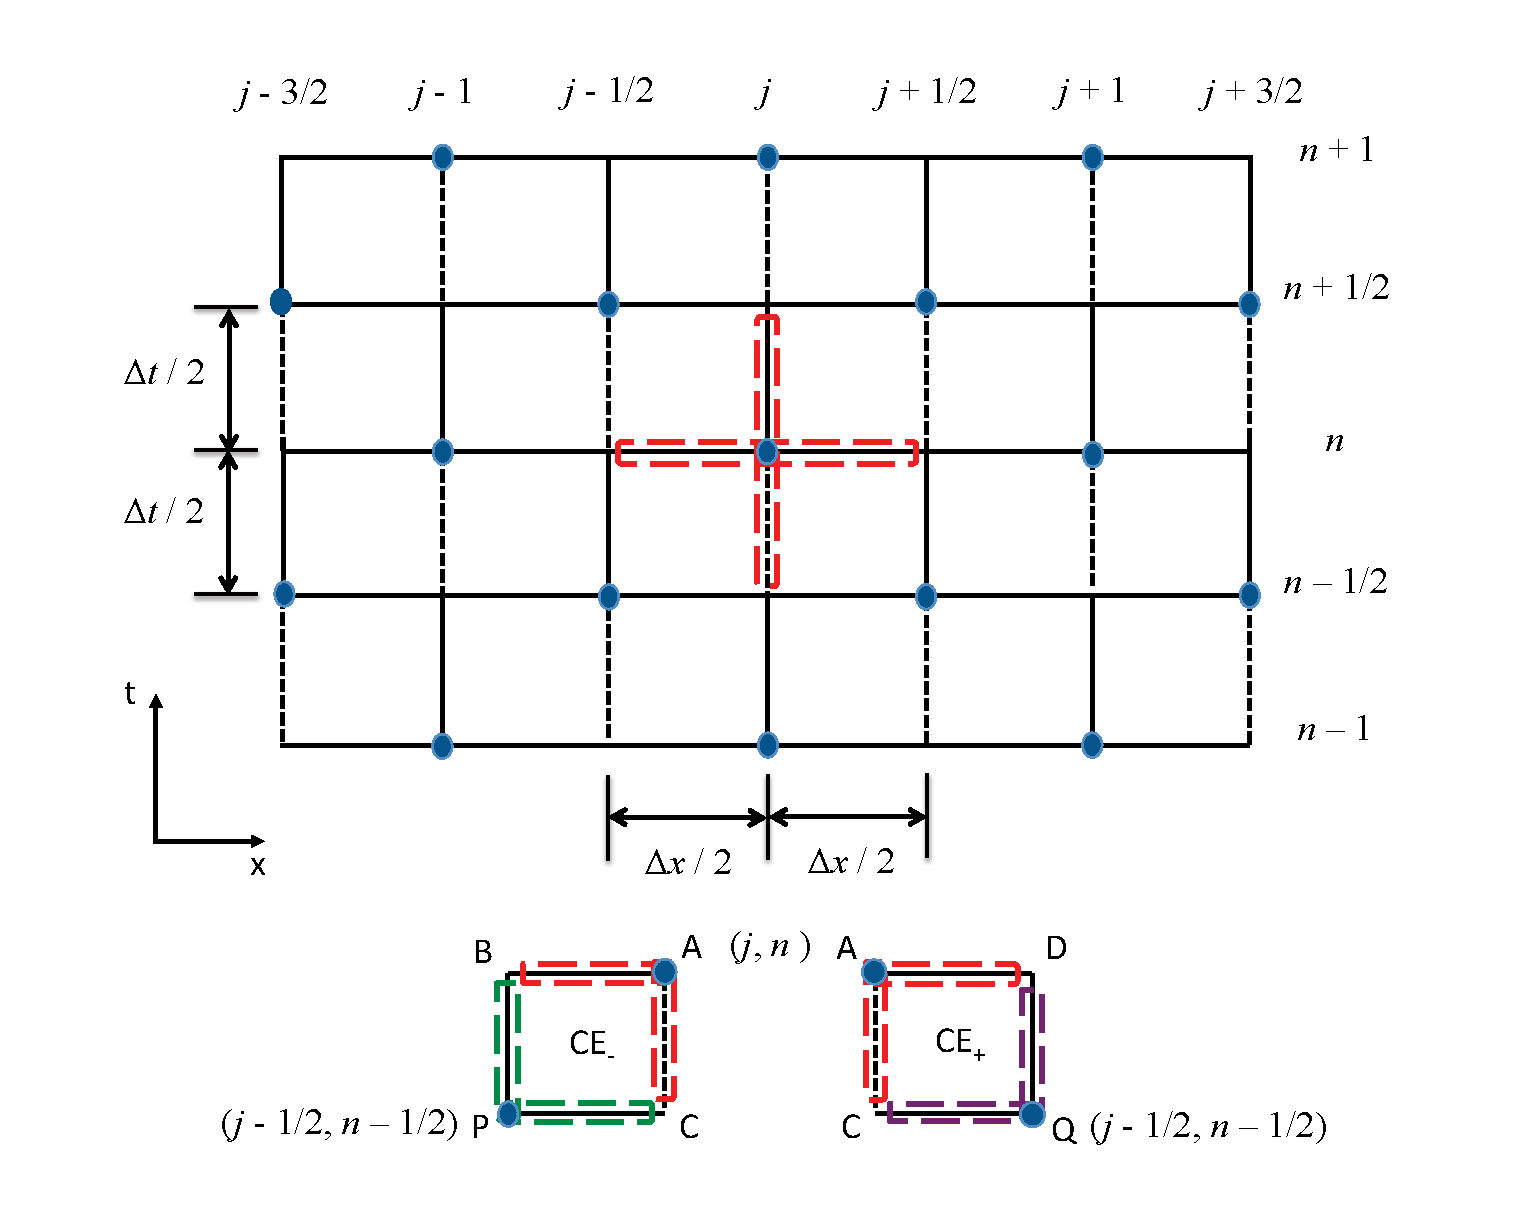
\includegraphics[width=0.8\textwidth]{mesh_and_ce_se_v1.eps}
      \caption{The mesh, conservation elements and solution elements. The cross
               -shaped region formed with red dash line is one of the solution
               element in the mesh.}
     \label{fig:mesh_and_ce_se_v1}
    \end{figure}

    \hspace{4mm}Eq.(2.6) $u^{*}(x,t;j,n)=u^{n}_{j}+(u_{x})^{n}_{j}[(x-x_{j})
                         -a(t-t^{n})], (x,t)\in SE(j,n)$

    \hspace{4mm}Eq.(2.9) $\vec{\bf{g}}^{*}\equiv
                         (-u^{*},au^{*}-\mu\partial u^{*}/\partial x)
                         , d{\bf{r}}\equiv(dx,dt)$

    \hspace{4mm}$F_{\pm}(j,n)=
                \oint^{c.c.}_{S(CE_{\pm}(j,n))}\vec{\bf{g}}^{*}\cdot d{\bf{r}}$

    \hspace{4mm}For CE$_{-}(ABPC)$ shown in Figure~\ref{fig:mesh_and_ce_se_v1}:

    \hspace{8mm}$\int^{B}_{A}\{-u^{n}_{j}-(u_{x})^{n}_{j}[(x-x_{j})-a(t-t^{n})]\}dx$

    \hspace{16mm}$=-u^{n}_{j}x|^{B}_{A}-\int^{B}_{A}(u_{x})^{n}_{j}(x-x_{j})(t-t^{n})
                 d(x-x_{j})+a(u_{x})^{n}_{j}(t-t^{n})x|^{B}_{A}$

    \hspace{16mm}$=\frac{\Delta x}{2}u^{n}_{j}
                 -\frac{(\Delta x)^{2}}{8}(u_{x})^{n}_{j}$

    \hspace{8mm}$\int^{P}_{B}\{au^{n-1/2}_{j-1/2}+a(u_{x})^{n-1/2}_{j-1/2}
                [(x-x_{j-1/2})-a(t-t^{n-1/2})]-\mu(u_{x})^{n-1/2}_{j-1/2}\}dt$

    \hspace{16mm}$=-a\frac{\Delta t}{2}u^{n-1/2}_{j-1/2}+
                 a^{2}\frac{(\Delta t)^{2}}{8}(u_{x})^{n-1/2}_{j-1/2}
                 +\mu(u_{x})^{n-1/2}_{j-1/2}$

    \hspace{8mm}$\int^{C}_{P}\{-u^{n-1/2}_{j-1/2}
                -(u_{x})^{n-1/2}_{j-1/2}[(x-x_{j-1/2})-a(t-t^{n-1/2})]\}dx$

    \hspace{16mm}$=-\frac{\Delta x}{2}u^{n-1/2}_{j-1/2}
                 -\frac{(\Delta x)^{2}}{8}(u_{x})^{n-1/2}_{j-1/2}$

    \hspace{8mm}$\int^{A}_{C}\{au^{n}_{j}+a(u_{x})^{n}_{j}[(x-x_{j})
                -a(t-t^{n})]-\mu(u_{x})^{n}_{j}\}$

    \hspace{16mm}$=a\frac{\Delta t}{2}u^{n}_{j}
                 +a^{2}\frac{(\Delta t)^{2}}{8}(u_{x})^{n}_{j}
                 -\mu\frac{\Delta t}{2}(u_{x})^{n}_{j}$

    \hspace{4mm}${}_\cdot{}^\cdot{}_\cdot~F_{-}(j,n)$

    \hspace{8mm}$=(-\frac{(\Delta x)^{2}}{8}+a^{2}\frac{(\Delta t)^{2}}{8}
                -\mu\frac{\Delta t}{2})(u_{x})^{n}_{j}
                +(-\frac{(\Delta x)^{2}}{8}+a^{2}\frac{(\Delta t)^{2}}{8}
                +\mu\frac{\Delta t}{2})(u_{x})^{n-1/2}_{j-1/2}
                +(\frac{\Delta x}{2}+a\frac{\Delta t}{2})u^{n}_{j}$

    \hspace{12mm}$+(-\frac{\Delta x}{2}-a\frac{\Delta t}{2})u^{n-1/2}_{j-1/2}$

    \hspace{8mm}$=(-\frac{1}{2})(\frac{(\Delta x)^{2}}{4})
                [(1-a^{2}\frac{(\Delta t)^{2}}{(\Delta x)^{2}}
                +4\mu\frac{\Delta t}{(\Delta x)^{2}})(u_{x})^{n}_{j}
                +(1-a^{2}\frac{(\Delta t)^{2}}{(\Delta x)^{2}}
                -4\mu\frac{\Delta t}{(\Delta x)^{2}})(u_{x})^{n-1/2}_{j-1/2}]$

    \hspace{12mm}$+\frac{(\Delta x)^{2}}{4}\frac{2}{\Delta x}
                 (1+a\frac{\Delta t}{\Delta x})(u^{n}_{j}-u^{n-1/2}_{j-1/2})$

    \hspace{4mm}$\Rightarrow\frac{4}{(\Delta x)^{2}}F_{-}(j,n)$

    \hspace{8mm}$=-(\frac{1}{2})[(1-\nu^{2}+\xi)(u_{x})^{n}_{j}+
                (1-\nu^{2}-\xi)(u_{x})^{n-1/2}_{j-1/2}]
                +\frac{2(1+\nu)}{\Delta x}(u^{n}_{j}-u^{n-1/2}_{j-1/2})$

    \hspace{12mm}, where $\nu\equiv\frac{a\Delta t}{\Delta x}$
                 and $\xi\equiv\frac{4\mu\Delta t}{(\Delta x)^{2}}$.

    \hspace{4mm}Similarly, $\frac{4}{(\Delta x)^{2}}F_{+}(j,n)$

    \hspace{8mm}$=+(\frac{1}{2})[(1-\nu^{2}+\xi)(u_{x})^{n}_{j}
                +(1-\nu^{2}-\xi)(u_{x})^{n-1/2}_{j+1/2}]
                +\frac{2(1-\nu)}{\Delta x}(u^{n}_{j}-u^{n-1/2}_{j+1/2})$

    \hspace{12mm}, where $\nu\equiv\frac{a\Delta t}{\Delta x}$
                 and $\xi\equiv\frac{4\mu\Delta t}{(\Delta x)^{2}}$.

  \item Derivation of Eq.(2.34) \newline
    $\psi(x,t;j,n)=-\frac{(u_{x})^{n}_{j}}{2}
    \{[(x-x_{j})-a(t-t^{n})]^{2}+2\mu(t-t^{n})\}-u^{n}_{j}[(x-x_{j})-a(t-t^{n})]$:

    \hspace{4mm}Eq.(2.6) $u^{*}=u^{n}_{j}+(u_{x})^{n}_{j}[(x-x_{j})-a(t-t{n})]$

    \hspace{4mm}Eq.(2.32) $\frac{\partial\psi}{\partial t}=au^{*}
                          -\mu\frac{\partial u^{*}}{\partial x}$

    \hspace{4mm}Eq.(2.33) $-\frac{\partial\psi}{\partial x}=u^{*}$
                , it should be noted that the original Eq.(2.33)
                listed in paper

    \hspace{4mm}is wrong.

    \hspace{4mm}By substituting Eq.(2.6) into Eq.(2.32), we can have:

    \hspace{8mm}$\psi=au^{n}_{j}(t-t^{n})+a(u_{x})^{n}_{j}(x-x_{j})(t-t^{n})
                -\frac{a^{2}}{2}(u_{x})^{n}_{j}(t-t^{n})^{2}
                -\mu(u_{x})^{n}_{j}(t-t^{n})+C(x)$

    \hspace{4mm}We then substitute the above result into Eq.(2.33):

    \hspace{8mm}$-a(u_{x})^{n}_{j}(t-t^{n})-C'(x)=u^{n}_{j}
                +(u_{x})^{n}_{j}[(x-x_{j})-a(t-t^{n})]$

    \hspace{4mm}$\Rightarrow C'(x)=-u^{n}_{j}-(u_{x})^{n}_{j}(x-x_{j})$

    \hspace{4mm}$\Rightarrow C(x)=-u^{n}_{j}(x-x_{j})
                -\frac{(u_{x})^{n}_{j}}{2}(x-x_{j})^{2}$

    \hspace{4mm}${}_\cdot{}^\cdot{}_\cdot~\psi=
                -\frac{(u_{x})^{n}_{j}}{2}[(x-x_{j})^{2}-2a(x-x_{j})(t-t^{n})
                +a^{2}(t-t^{n})^{2}+2\mu(t-t^{n})]-u^{n}_{j}[(x-x_{j})$

    \hspace{17mm}$-a(t-t^{n})]$

    \hspace{12mm}$=-\frac{(u_{x})^{n}_{j}}{2}\{[(x-x_{j})-a(t-t^{n})]^{2}
                 +2\mu(t-t^{n})\}-u^{n}_{j}[(x-x_{j})-a(t-t^{n})]$

  \item Derivation of Eq.(4.20) \newline
    $\psi_{m}=(f_{m})^{n}_{j}(t-t^{n})-(u_{m})^{n}_{j}(x-x_{j})
    +\frac{1}{2}(f_{m})^{n}_{j}(t-t^{n})^{2}
    -\frac{1}{2}(u_{mx})^{n}_{j}(x-x_{j})^{2}
    +(f_{mx})^{n}_{j}(x-x_{j})(t-t^{n})$:

    \hspace{4mm}By substituting Eq.(4.14) into Eq.(4.18), we can have:

    \hspace{8mm}$\frac{\partial\psi_{m}}{\partial t}=(f_{m})^{n}_{j}
                +(f_{mx})^{n}_{j}(x-x_{j})+(f_{mt})^{n}_{j}(t-t^{n})$

    \hspace{4mm}$\Rightarrow\psi_{m}=(f_{m})^{n}_{j}(t-t^{n})
                +(f_{mx})^{n}_{j}(x-x_{j})(t-t^{n})
                +\frac{1}{2}(f_{mt})^{n}_{j}(t-t^{n})^{2}+C(x)$
                --- \text{\textcircled{1}}

    \hspace{4mm}Similarly, by substituting Eq.(4.9) into Eq.(4.19), we can have:

    \hspace{8mm}$-\frac{\partial\psi_{m}}{\partial x}=(u_{m})^{n}_{j}
                +(u_{mx})^{n}_{j}(x-x_{j})+(u_{mt})^{n}_{j}(t-t^{n})$
                --- \text{\textcircled{2}}

    \hspace{4mm}Then we substitute Eq.\text{\textcircled{1}}
                into Eq.\text{\textcircled{2}}:

    \hspace{8mm}$-(f_{mx})^{n}_{j}(t-t^{n})-C'(x)=(u_{m})^{n}_{j}
                +(u_{mx})^{n}_{j}(x-x_{j})+(u_{mt})^{n}_{j}(t-t^{n})$

    \hspace{4mm}$\Rightarrow C(x)=-(f_{mx})^{n}_{j}(x-x_{j})(t-t^{n})
                -(u_{m})^{n}_{j}(x-x_{j})
                -\frac{1}{2}(u_{mx})^{n}_{j}(x-x_{j})^{2}$

    \hspace{12mm}$-(u_{mt})^{n}_{j}(x-x_{j})(t-t^{n})$

    \hspace{4mm}${}_\cdot{}^\cdot{}_\cdot~\psi_{m}=(f_{m})^{n}_{j}(t-t^{n})
                +(f_{mx})^{n}_{j}(x-x_{j})(t-t^{n})
                +\frac{1}{2}(f_{mt})^{n}_{j}(t-t^{n})^{2}-(f_{mx})^{n}_{j}(x-$

    \hspace{20mm}$x_{j})(t-t^{n})-(u_{m})^{n}_{j}(x-x_{j})
                 -\frac{1}{2}(u_{mx})^{n}_{j}(x-x_{j})^{2}
                 -(u_{mt})^{n}_{j}(x-x_{j})(t-t^{n})$

    \hspace{4mm}${}^\cdot{}_\cdot{}^\cdot$
                Eq.(4.17) $(u_{mt})^{n}_{j}=-(f_{mx})^{n}_{j}$

    \hspace{4mm}${}_\cdot{}^\cdot{}_\cdot~\psi_{m}=(f_{m})^{n}_{j}(t-t^{n})
                -(u_{m})^{n}_{j}(x-x_{j})+\frac{1}{2}(f_{m})^{n}_{j}(t-t^{n})^{2}
                -\frac{1}{2}(u_{mx})^{n}_{j}(x-x_{j})^{2}+(f_{mx})^{n}_{j}(x-$

    \hspace{20mm}$x_{j})(t-t^{n})$
 \end{enumerate}

\section{How to develop our own CESE solver}
 \label{sec:development_cese}
By referring to the paper "The Method of Space-Time Conservation Element and 
Solution Element -- A New Approach for Solving the Navier-Stokes and Euler 
Equations."~\cite{CESE_Shin_Chung_Chang_1995}, the CESE solver provided in this 
note basically is build with Python 2.7. But It should be noted the original 
paper of CESE method also attach an example code in its appendix, which is 
written in Fortran. 

Necessary or recommended libraries which are used in our implementation of CESE
method:
 \begin{enumerate}
  \item Numpy, a fundamental package for scientific computing with Python.
  \item matplotlib, a python plotting library.
 \end{enumerate}
Useful tools:
 \begin{enumerate}
  \item PyCharm, a power python IDE (integrated development environment).
  \item iPython, an interactive computational environment.
 \end{enumerate}
Next, we demonstrate how we implement CESE solver for solving this 
one-dimensional shock tube problem in Python.

\subsection{One-dimensional shock tube problem}
 \label{sec:1d_shock_tube}
The one-dimensional Sod shock tube problem is widely employed for testing 
computational fluid programs. Figure~\ref{fig:sod_shock_tube_1D} shows the
initial conditions of different regions in our Sod shock tube. The whole
one-dimension space is separated into two regions by a diaphragm in the
beginning. The gas is the same in both regions. The left region is called
driven section and containing the gas with the higher density $\rho_l$ and
the higher pressure $p_l$. The right region is called working section and
with the gas at the lower density $\rho_r$ and the lower pressure $p_r$.
Before removing the diaphragm, the gas in both regions is static. The global
specific heat ratio ($\gamma\buildrel{\text{def}}\over{=}\frac{c_p}{c_v}$)
is 1.4.

 \begin{figure}[hbtp]
    \centering
     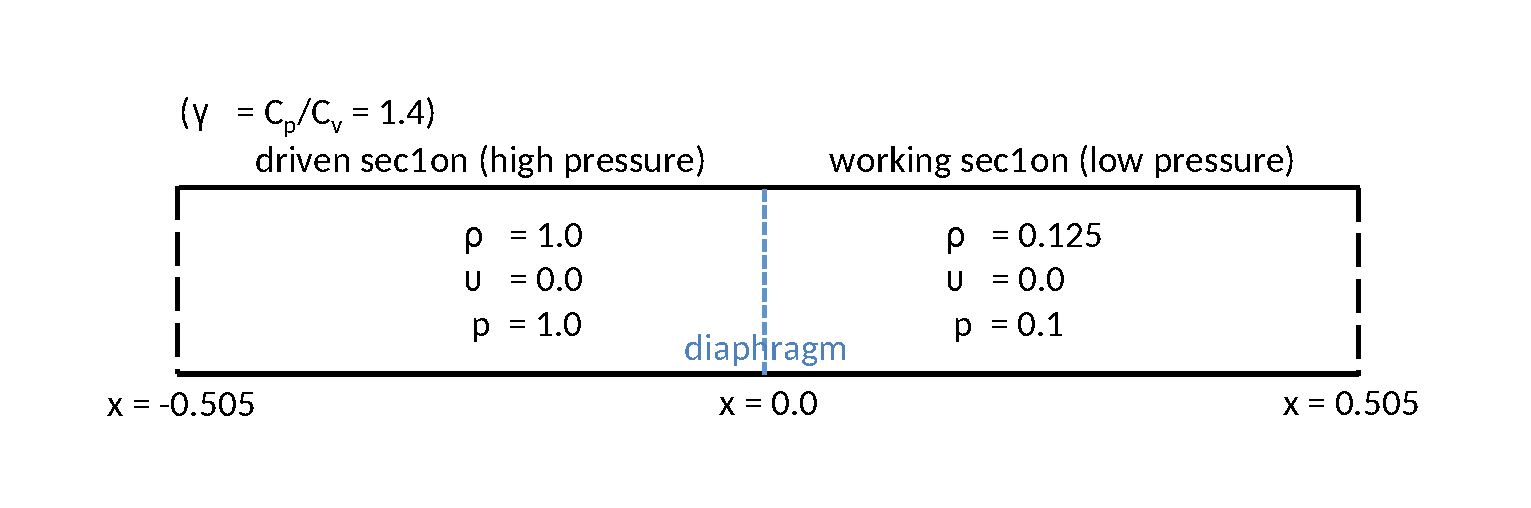
\includegraphics[width=0.8\textwidth]{sod_shock_tube_1D.eps}
     \caption{Initial condition of one-dimensional Sod shock tube}
     \label{fig:sod_shock_tube_1D}
 \end{figure}

When the diaphragm is removed from the tube, there is a right-running shock in 
working section; meanwhile, there is a rarefaction wave in the driven section as
described in Figure~\ref{fig:sod_shock_tube_1D_no_diaphragm}. Basically, 
through implementing the CESE method here, we can quite easily calculate the 
status $(\rho, \nu, p)$ of different regions.

 \begin{figure}[hbtp]
    \centering
     \includegraphics[width=0.8\textwidth]{sod_shock_tube_1D_no_diaphragm.eps}
     \caption{Waves propagating in the tube after the removal of the diaphragm}
     \label{fig:sod_shock_tube_1D_no_diaphragm}
 \end{figure}

The tube is infinitely long and we focus on the region between -0.505 and 0.505.
According to the presetting of the CESE method, we then design a mesh to 
calculate the gas status in different regions as time goes on. The size of each 
grid element or so-called conservation element is $(dx/2, dt/2)$, where $dx$ is 
0.01 and $dt$ is 0.004. The whole one-dimensional space (-0.505$\sim$0.505) is 
then divided into 101 segments by 102 points or so-called solution elements.
Figure~\ref{fig:mesh_and_ce_v2} shows the configuration of the mesh we set for 
the one-dimension Sod shock tube problem.

 \begin{figure}[ht]
    \centering
     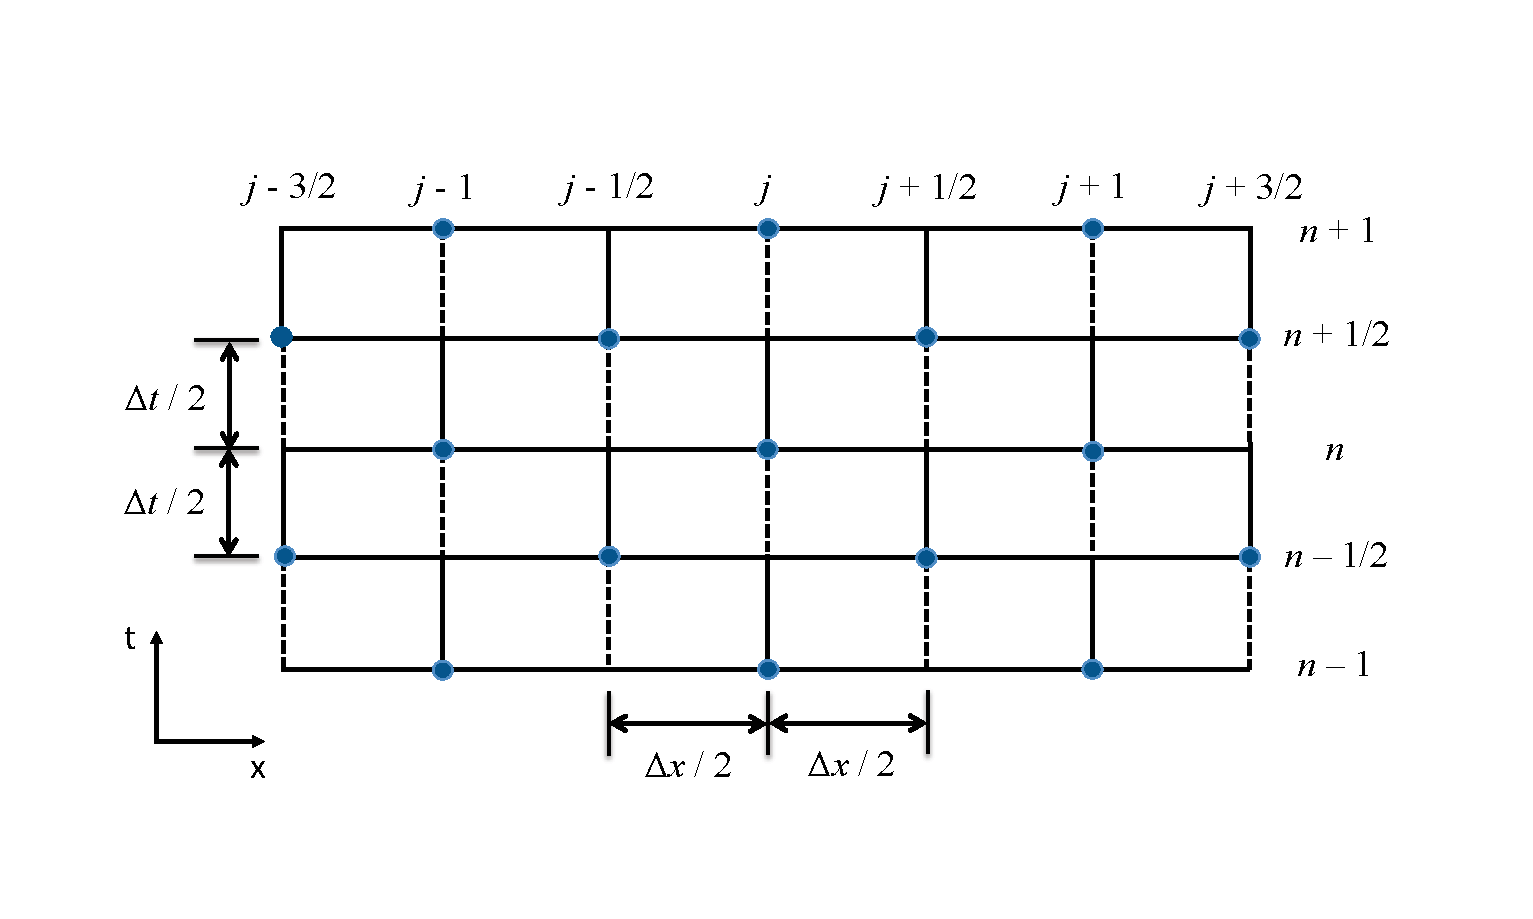
\includegraphics[width=0.8\textwidth]{mesh_and_ce.eps}
     \caption{The mesh and conservation elements.}
     \label{fig:mesh_and_ce_v2}
 \end{figure}

The future status of gas in each position can be evaluated by using the 
information of its previous status. That is, if the shock tube starts to evolve 
at $t=t^{n-1}$, we can extract the status of gas at $t=t^{n-1/2}$ through one 
numerical calculation.
Here, we attempt to evaluate the status of gas for all $n$ with $t^{n}\leq0.2$
and then we can compare our results with analytic solution and also those shown
in Section 7 of Prof. S. C. Chang's CESE paper~\cite{CESE_Shin_Chung_Chang_1995}.
Obviously, we evaluate the status of gas by using CESE method iteratively.
There are 100 times of iteration in our for loop.

For efficiency concern, we choose a widely used Pyton package 'Numpy' for all of 
the matrix calculations. We then create many of asymmetric matrices for different 
usages. Table~\ref{tab:mtx_comparision} shows the relationship between matrices 
in Python code and those in section 4 of Prof. S. C. Chang's CESE 
paper~\cite{CESE_Shin_Chung_Chang_1995}.
It should be noted that both 'mtx\_q' and 'mtx\_qn' are used to stored the
information of $(u_{m})^{n}_{j}$. The only difference is that 'mtx\_q' is for
current status of gas while 'mtx\_qn' is for the status of gas after one time
iteration ($dt/2$).

\begin{table*}[ht]
\begin{center}
\caption{Comparison table of matrices in Python code and matrices in paper.
        \label{tab:mtx_comparision}}
\begin{tabular}{l|l}
\hline\hline
Python code         & Paper \\\hline
mtx\_f              & $f_{m,k}$ \\
mtx\_q, mtx\_qn     & $(u_{m})^{n}_{j}$ \\
mtx\_qx             & $(u_{kx})^{n}_{j}$ \\
mtx\_qt             & $(u_{mt})^{n}_{j}$ \\
mtx\_s              & $(s_{m})^{n}_{j}$ \\
uxl                 & $(u_{mx-})^{n}_{j}$ \\
uxr                 & $(u_{mx+})^{n}_{j}$ \\
\hline\hline
\end{tabular}
\end{center}
\end{table*}

Now let's start to use CESE method for solving this shock tube problem.
The calculation can be divided into many steps in each iteration.

\subsubsection{First step}
 \label{subsubsec:first_step}
First, we have to extract some necessary information from the current status
of gas. By referring to Eq.(4.7) of~\cite{CESE_Shin_Chung_Chang_1995},
\begin{equation}
f_{m,k}\equiv\partial f_{m}/\partial u_{k},~m,~k = 1,~2,~3
\end{equation}
we can easily have the Jacobian matrix $F$ of $f_{m,k}$:
\begin{equation}
\begin{array}{l}
F\equiv\left[
       \begin{array}{ccc}
       f_{1,1} & f_{1,2} & f_{1,3} \\
       f_{2,1} & f_{2,2} & f_{2,3} \\
       f_{3,1} & f_{3,2} & f_{3,3}
       \end{array}
       \right]
       =
       \left[
       \begin{array}{ccc}
       \frac{\partial f_{1}}{\partial u_{1}} & \frac{\partial f_{1}}{\partial
       u_{2}} & \frac{\partial f_{1}}{\partial u_{3}} \\ \\
       \frac{\partial f_{2}}{\partial u_{1}} & \frac{\partial f_{2}}{\partial
       u_{2}} & \frac{\partial f_{2}}{\partial u_{3}} \\ \\
       \frac{\partial f_{3}}{\partial u_{1}} & \frac{\partial f_{3}}{\partial
       u_{2}} & \frac{\partial f_{3}}{\partial u_{3}}
       \end{array}
       \right] \\ \\
       \hspace{44mm}=
       \left[
       \begin{array}{ccc}
       0 & 1 & 0 \\
       \frac{\gamma -3}{2}\frac{u^{2}_{2}}{u^{2}_{1}} & -(\gamma -3)\frac{u_{2}}
       {u_{1}} & \gamma -1 \\
       (\gamma -1)\frac{u^{3}_{2}}{u^{3}_{1}}-\gamma\frac{u_{2}u_{3}}{u^{2}_{1}}
       & \gamma\frac{u_{3}}{u_{1}}-\frac{3}{2}(\gamma -1)\frac{u^{2}_{2}}{u^{2}_{1}}
       & \gamma\frac{u_{2}}{u_{1}}
       \end{array}
       \right]
\end{array}
\end{equation}
where $u_{1}\equiv\rho,~u_{2}\equiv\rho\nu,~u_{3}\equiv\frac{p}{\gamma -1}
+\frac{1}{2}\rho\nu^{2},$ \newline
and $f_{1}\equiv u_{2},~f_{2}\equiv(\gamma -1)u_{3}+\frac{3-\gamma}{2}
\frac{u^{2}_{2}}{u_{1}},~f_{3}\equiv\gamma\frac{u_{2}u_{3}}{u_{1}}
-\frac{\gamma -1}{2}\frac{u^{3}_{2}}{u^{2}_{1}}$. \newline
Also, with the aid of Eq.(4.12), Eq.(4.17) and Eq.(4.25)
of~\cite{CESE_Shin_Chung_Chang_1995}, we then can evaluate $(u_{mt})^{n}_{j}$
and $(s_{m})^{n}_{j}$:
\begin{equation}
(u_{mt})^{n}_{j} = -(f_{mx})^{n}_{j} = -(f_{m,k}u_{kx})^{n}_{j}
\end{equation}
\begin{equation}
(s_{m})^{n}_{j}\equiv\frac{\Delta x}{4}(u_{mx})^{n}_{j}+\frac{\Delta t}
{\Delta x}(f_{m})^{n}_{j}+\frac{(\Delta t)^{2}}{4\Delta x}(f_{m})^{n}_{j}
,~m=1,~2,~3
\end{equation}

The corresponding Python code can be implemented as follows, where index 'j' is 
the index of for loop. The for loop goes through specific elements of matrix 
with respect to varying intervals:
\begin{pythonNoIndex}
                            .
                            .
                            .
        w2 = mtx_q[1, j] / mtx_q[0, j]  # u2/u1
        w3 = mtx_q[2, j] / mtx_q[0, j]  # u3/u1
        mtx_f[0, 0] = 0.0
        mtx_f[0, 1] = 1.0
        mtx_f[0, 2] = 0.0
        mtx_f[1, 0] = -0.5 * (3.0 - ga) * w2**2
        mtx_f[1, 1] = (3.0 - ga) * w2
        mtx_f[1, 2] = ga - 1.0
        mtx_f[2, 0] = (ga - 1.0) * w2**3 - ga * w2 * w3
        mtx_f[2, 1] = ga * w3 - 1.5 * (ga - 1.0) * w2**2
        mtx_f[2, 2] = ga * w2

        mtx_qt[:,j] = -1.0 * mtx_f * mtx_qx[:,j]

        mtx_s[:, j] = 0.25 * dx * mtx_qx[:, j] + (dt / dx) * mtx_f * mtx_q[:,j] \
                          - 0.25 * dt * (dt / dx) * mtx_f * mtx_f * mtx_qx[:,j]
                            .
                            .
                            .
\end{pythonNoIndex}

It's worth to pay attention to the loop range of the above calculation.
Instead of keeping visiting every position from the beginning, we choose a
different way to construct this for loop. From the essence of this shock tube
problem, changes of gas statuses happen from the center of the tube (contact
discontinuity) to both sides as time goes on after removing the diaphragm.
These calculations focus on the central two SE points in first loop. Then the
range of loop will be increased by one point on each side every two loop. 
That is, the central four points will be visited in next loop. But actually this
modification won't decrease the space complexity too much. It still takes
$O(n^{2})$ as if we start to loop every position from the beginning.

\subsubsection{Second step}
 \label{subsubsection:second_step}
Next, we evaluate the future status of gas after time stamp moves forward
by $dt/2$. By referring to Eq.(4.24) of~\cite{CESE_Shin_Chung_Chang_1995}, the
status of gas after $dt/2$ can be evaluated through the its current status.
\begin{equation}
(u_{m})^{n}_{j}=\frac{1}{2}[(u_{m})^{n-1/2}_{j-1/2}+(u_{m})^{n-1/2}_{j+1/2}
+(s_{m})^{n-1/2}_{j-1/2}-(s_{m})^{n-1/2}_{j+1/2}],~m=1,~2,~3
\end{equation}

Besides, we also need to calculate $(u_{mx})^{n}_{j}$ for the next iteration by
using the current and the future status of gas. In order to achieve this goal, 
Eq.(4.27), Eq.(4.36), Eq.(4.38) and Eq.(4.39) 
of ~\cite{CESE_Shin_Chung_Chang_1995} play very important roles here.
\begin{equation}
(u'_{m})^{n}_{j\pm1/2}\equiv(u_{m})^{n-1/2}_{j\pm1/2}
+\frac{\Delta t}{2}(u_{mt})^{n-1/2}_{j\pm1/2}
\end{equation}
\begin{equation}
(u_{mx\pm})^{n}_{j}\equiv\frac{(u'_{m})^{n}_{j\pm1/2}-(u_{m})^{n}_{j}}{\Delta x/2}
,~m=1,~2,~3
\end{equation}
\begin{equation}
(u^{W_{0}}_{mx})^{n}_{j}\equiv W_{0}((u_{mx-})^{n}_{j},(u_{mx+})^{n}_{j};\alpha)
,~m=1,~2,~3
\end{equation}
Here $\alpha$ is an adjustable constant for weighting and the function $W_{0}$
is defined by (i) $W_{0}(0, 0, \alpha)=0$ and (ii)
\begin{equation}
W_{0}(x_{-},x_{+};\alpha )=\frac{|x_{+}|^{\alpha}x_{-}+|x_{-}|^{\alpha}x_{+}}
{|x_{+}|^{\alpha}+|x_{+-}|^{\alpha}},~(|x_{+}|+|x_{-}|>0),
\end{equation}
where $x_{+}$ and $x_{-}$ are any two real variables.

As mentioned in~\cite{CESE_Shin_Chung_Chang_1995}, this method develops weighted 
average instead of using the central-difference approximation for 
$\partial u_{m}/\partial x$. 
This weighted average is valid even in the presence of discontinuity. It should
be noted that we set the weighting factor $\alpha$ to be '1' in this solver.

The corresponding Python code is here, where index 'j' is the index of the for 
loop. It goes through specific elements of matrix according to the varying
intervals. The range of this for loop is very similar to the one shown in the 
first step.
\begin{pythonNoIndex}
                            .
                            .
                            .
        mtx_qn[:, j+1] = 0.5 * (mtx_q[:, j] + mtx_q[:, j+1] + mtx_s[:, j] - mtx_s[:, j+1])
        uxl = np.asarray((mtx_qn[:, j+1] - mtx_q[:, j] - 0.5 * dt * mtx_qt[:, j]) \
                                                                    / (dx / 2.0))
        uxr = np.asarray((mtx_q[:, j+1] + 0.5 * dt * mtx_qt[:, j+1] - mtx_qn[:, j+1]) \
                                                                        / (dx / 2.0))
        mtx_qx[:, j+1] = np.asmatrix((uxl * (abs(uxr))**weight + uxr * (abs(uxl))**weight) \
                                      / ((abs(uxl))**weight + (abs(uxr))**weight + 10**(-60)))
                            .
                            .
                            .
\end{pythonNoIndex}

\subsubsection{Third step}
 \label{subsubsec:third_step}
Basically, all of the needed calculations of the CESE method for evaluating the 
status of gas in each iteration is done by the previous two steps.
The rest thing is to reset the information of position which is stored in 
'mtx\_q' for next iteration.
Hence, the information stored in 'mtx\_qn' will be assigned back to 'mtx\_q'.
It should be noted that both 'mtx\_q' and 'mtx\_qx' have to be translated 
backward 1 dx per 1 dt (2 iterations). 
This is simply due to the nature of the CESE method and also the matrix operation 
in our program. After that, it's time to export the results for visualization.
The complete Python code of CESE solver can be found in 
Section~\ref{subsec:python_code}.

\subsection{Python code}
 \label{subsec:python_code}
\begin{pythonWithIndex}
import matplotlib
matplotlib.use('TKAgg')

import numpy as np
import matplotlib.pyplot as plt
import matplotlib.animation as animation

# global variable
it = 100            # number of iterations
npx = it + 2        # number of points (x-axis)
dt = 0.4 * 10**(-2) # time interval = 0.004
dx = 0.1 * 10**(-1) # space interval = 0.01
ga = 1.4            # gamma = Cp/Cv

rhol = 1.0
pl   = 1.0
vl   = 0.0
rhor = 0.125
pr   = 0.1
vr   = 0.0

weight = 1 # weighting factor of Eq.(4.39)

# necessary matrices for CESE calculation
mtx_q  = np.asmatrix(np.zeros(shape=(3, npx)))
mtx_qn = np.asmatrix(np.zeros(shape=(3, npx)))
mtx_qx = np.asmatrix(np.zeros(shape=(3, npx)))
mtx_f  = np.asmatrix(np.zeros(shape=(3, 3)))
mtx_qt = np.asmatrix(np.zeros(shape=(3, npx)))
mtx_s  = np.asmatrix(np.zeros(shape=(3, npx)))
uxl = np.zeros(shape=(3,1))
uxr = np.zeros(shape=(3,1))

# output lists
xx  = [0. for idx in range(npx)] # x-axis
status_rho  = [rhor if idx >= npx / 2 else rhol for idx in range(npx)] # rho
status_vel  = [0. for idx in range(npx)] # v
status_p  = [pr if idx >= npx / 2 else pl for idx in range(npx)] # p

# initialization of matrix u
for j in xrange(0, npx):
    # Eq (4.1), u1, u2 and u3
    if j < npx / 2:
        mtx_q[0, j] = rhol
        mtx_q[1, j] = rhol * vl
        mtx_q[2, j] = pl / (ga - 1.0) + 0.5 * rhol * vl**2
    else:
        mtx_q[0, j] = rhor
        mtx_q[1, j] = rhor * vr
        mtx_q[2, j] = pr / (ga - 1.0) + 0.5 * rhor * vr**2

# setting the x-axis, from -0.505 to 0.505
xx[0] = -0.5 * dx * float(it + 1)
for j in xrange(0, npx - 1):
    xx[j+1] = xx[j] + dx

# initialization of output plots
fig = plt.figure()
frame_seq = []

# variables of loop
mtx_length = npx
start_point = npx / 2 - 1
stepping = 2

# start to evaluate the solution iteratively
for i in xrange(0, it):

    # evaluate the current status of gas
    for j in xrange(start_point, start_point + stepping):

        # Eq. (4.7): constructing the matrix fm,k
        # other reference: Yung-Yu's notes -> Sec.3.1, Eq. (3.14)
        w2 = mtx_q[1, j] / mtx_q[0, j]  # u2/u1
        w3 = mtx_q[2, j] / mtx_q[0, j]  # u3/u1
        mtx_f[0, 0] = 0.0
        mtx_f[0, 1] = 1.0
        mtx_f[0, 2] = 0.0
        mtx_f[1, 0] = -0.5 * (3.0 - ga) * w2**2
        mtx_f[1, 1] = (3.0 - ga) * w2
        mtx_f[1, 2] = ga - 1.0
        mtx_f[2, 0] = (ga - 1.0) * w2**3 - ga * w2 * w3
        mtx_f[2, 1] = ga * w3 - 1.5 * (ga - 1.0) * w2**2
        mtx_f[2, 2] = ga * w2

        # Eq.(4.17), (u_mt)nj = -(f_mx)nj = -(fm,k*u_kx)nj, (u_mt)nj -> qt, (u_kx)nj -> qx
        mtx_qt[:,j] = -1.0 * mtx_f * mtx_qx[:,j]

        # Eq.(4.25), (u_m)nj -> q, (u_mt)nj -> qt, (u_kx)nj -> qx
        mtx_s[:, j] = 0.25 * dx * mtx_qx[:, j] + (dt / dx) * mtx_f * mtx_q[:,j] \
                          - 0.25 * dt * (dt / dx) * mtx_f * mtx_f * mtx_qx[:,j]

    # evaluate the status of gas after time stamp moves forward by 1 dt/2
    ssm1 = start_point + stepping - 1
    for j in xrange(start_point, ssm1): # j -> 1 dx/2
        # Eq.(4.24), 'qn' = the next state of 'q',
        # where (u_m)nj -> qn, (u_m)(n-1/2)(j+-1/2) -> q
        mtx_qn[:, j+1] = 0.5 * (mtx_q[:, j] + mtx_q[:, j+1] + mtx_s[:, j] - mtx_s[:, j+1])
        # Eq.(4.27) and Eq.(4.36), 'l' means '-' and 'r' means '+'.
        uxl = np.asarray((mtx_qn[:, j+1] - mtx_q[:, j] - 0.5 * dt * mtx_qt[:, j]) \
                                                                    / (dx / 2.0))
        uxr = np.asarray((mtx_q[:, j+1] + 0.5 * dt * mtx_qt[:, j+1] - mtx_qn[:, j+1]) \
                                                                        / (dx / 2.0))
        # Eq.(4.38) and Eq.(4.39)
        mtx_qx[:, j+1] = np.asmatrix((uxl * (abs(uxr))**weight + uxr * (abs(uxl))**weight) \
                                      / ((abs(uxl))**weight + (abs(uxr))**weight + 10**(-60)))

    for j in xrange(start_point + 1, start_point + stepping):
        mtx_q[:, j] = mtx_qn[:, j]

    # IMPORTANT: mtx_q and mtx_qx have to be translated backward 1 dx per 1 dt (2 iterations)
    if i % 2 != 0:
        for j in xrange(1, mtx_length):
            mtx_q[:, j-1] = mtx_q[:, j]
            mtx_qx[:, j-1] = mtx_qx[:, j]

        start_point -= 1
        stepping += 2

        # output region
        for j in xrange(0, mtx_length):
            status_rho[j] = mtx_q[0, j]
            status_vel[j] = mtx_q[1, j] / mtx_q[0, j]
            status_p[j] = (ga - 1.0) * (mtx_q[2, j] - 0.5 * mtx_q[0, j] * status_vel[j]**2)

        # making plots of gas status for different time intervals
        plt.subplot(311)
        plot_rho = plt.scatter(xx, status_rho, color="r")
        plt.xlabel("x")
        plt.ylabel("density")
        plt.xlim(-0.55, 0.55)
        plt.ylim(-0.1, 1.1)
        plt.subplot(312)
        plot_vel = plt.scatter(xx, status_vel, color="g")
        plt.xlim(-0.55, 0.55)
        plt.ylim(-0.1, 1.1)
        plt.xlabel("x")
        plt.ylabel("velocity")
        plt.subplot(313)
        plot_p = plt.scatter(xx, status_p, color="b")
        plt.xlim(-0.55, 0.55)
        plt.ylim(-0.1, 1.1)
        plt.xlabel("x")
        plt.ylabel("pressure")
        frame_seq.append((plot_rho, plot_vel, plot_p))

    # output text files which contain gas status of each point for different time intervals
    file = open("%03d" % (i + 1) + ".dat", 'w')
    for j in xrange(0, mtx_length):
        file.write(str(xx[j]) + " " + str(status_rho[j]) + " " + str(status_vel[j]) \
                                                   + " " + str(status_p[j]) + "\n")

    file.close()

ani = animation.ArtistAnimation(fig, frame_seq, interval=25, repeat_delay=300, blit=True)
ani.save('mySodTube.mp4', fps=10);

plt.show()
\end{pythonWithIndex}

\section{Progress report}
 \label{sec:progress_report}
 \begin{enumerate}
  \item ( - 20151211) reading the CESE paper~\cite{CESE_Shin_Chung_Chang_1995},
        Achievement: Section 2 and 3.
  \item (20151212 - 20160109) starting to focus on Euler solver and make my own
        1-D solver which is referred to Tai-Hsiang's code and appendix B of the
        CESE paper~\cite{CESE_Shin_Chung_Chang_1995}
  \item (20160110 - 20160314) finished the first version of CESE solver for 1-D
        sod shock tube problem. Starting to work on unit test and improve code
        structure.
  \item (20160707 - ) keep working on improving note.
 \end{enumerate}



\begin{thebibliography}{99}
\bibitem{CESE_Shin_Chung_Chang_1995} Sin-Chung Chang, The Method of Space-Time
         Conservation Element and Solution Element—A New Approach for Solving
         the Navier-Stokes and Euler Equations. Journal of Computational
         Physics, 119, 295-324, 1995.
\end{thebibliography}

\end{document}
